
\documentclass[12pt,journal,compsoc]{IEEEtran}
%
% If IEEEtran.cls has not been installed into the LaTeX system files,
% manually specify the path to it like:
% \documentclass[12pt,journal,compsoc]{../sty/IEEEtran}


% *** CITATION PACKAGES ***
%
\ifCLASSOPTIONcompsoc
\else
\fi

\ifCLASSINFOpdf
\else
\fi


\usepackage{url}
\usepackage{graphicx}
\usepackage{multirow}

\hyphenation{Web-GL-Viewer Web-GL Web-RTC}

\usepackage{color}
\definecolor{lightgray}{rgb}{0.9,0.9,0.9}

\usepackage{listings} % Listings Code taken from: http://stackoverflow.com/questions/741985/latex-source-code-listing-like-in-professional-books
  \usepackage{courier}
 \lstset{
         basicstyle=\footnotesize\ttfamily, % Standardschrift
         %numbers=left,               % Ort der Zeilennummern
         numberstyle=\tiny,          % Stil der Zeilennummern
         %stepnumber=2,               % Abstand zwischen den Zeilennummern
         numbersep=5pt,              % Abstand der Nummern zum Text
         tabsize=2,                  % Groesse von Tabs
         extendedchars=true,         %
         breaklines=true,            % Zeilen werden Umgebrochen
         keywordstyle=\color{red},
    		frame=b,         
 %        keywordstyle=[1]\textbf,    % Stil der Keywords
 %        keywordstyle=[2]\textbf,    %
 %        keywordstyle=[3]\textbf,    %
 %        keywordstyle=[4]\textbf,   \sqrt{\sqrt{}} %
         stringstyle=\color{white}\ttfamily, % Farbe der String
         showspaces=false,           % Leerzeichen anzeigen ?
         showtabs=false,             % Tabs anzeigen ?
         xleftmargin=17pt,
         framexleftmargin=17pt,
         framexrightmargin=5pt,
         framexbottommargin=4pt,
         backgroundcolor=\color{lightgray},
         showstringspaces=false      % Leerzeichen in Strings anzeigen ?        
 }
 
   %\captionsetup[lstlisting]{singlelinecheck=false, labelfont={blue}, textfont={blue}}
  \usepackage{caption}
\DeclareCaptionFont{white}{\color{white}}
\DeclareCaptionFormat{listing}{\colorbox[cmyk]{0.43, 0.35, 0.35,0.01}{\parbox{0.485\textwidth}{\hspace{15pt}#1#2#3}}}
\captionsetup[lstlisting]{format=listing,labelfont=white,textfont=white, singlelinecheck=false, margin=0pt, font={bf,footnotesize}}



\begin{document}


\title{WebGL on Mobile Devices}


\author{William~Almnes,~\IEEEmembership{University~of~Oslo}\\
        Marko~Andjic,~\IEEEmembership{University~of~Oslo}\\
        Matthias~Armbruster~\IEEEmembership{University~of~Mannheim}\\  
        and~Paul~Steinhilber,~\IEEEmembership{University~of~Mannheim}% <-this % stops a space

\IEEEcompsocitemizethanks{\IEEEcompsocthanksitem William W. F. Almnes: wwalmnes@student.matnat.uio.no}
\IEEEcompsocitemizethanks{\IEEEcompsocthanksitem Marko Andjic: marko.andjic@usit.uio.no}
\IEEEcompsocitemizethanks{\IEEEcompsocthanksitem Matthias Armbruster: marmbrus@rumms.uni-mannheim.de}
\IEEEcompsocitemizethanks{\IEEEcompsocthanksitem Paul R. E. Steinhilber: ps@paulsteinhilber.de}
\IEEEcompsocitemizethanks{\IEEEcompsocthanksitem Daniel Sch\"{o}n: schoen@informatik.uni-mannheim (advisor)}
\thanks{Submitted just before April 23, 2012.}}


\markboth{Joint Teleseminar 2012}%
{Shell \MakeLowercase{\textit{et al.}}: Bare Demo of IEEEtran.cls for Computer Society Journals}

\IEEEcompsoctitleabstractindextext{%
\begin{abstract}
Augmented Reality (AR) is not a completely new concept but it has in recent years, slowly but steadily, been gaining in popularity as the use and development of smartphones exploded. Relevant digital information layered on top of the user’s view has given us a new paradigm in the information use and interaction, and we have already seen new types of AR dedicated devices being introduced. WebGL, on the other hand, is a graphic library based on well-known OpenGL ES standard that opens the possibility for native 3D animations in a browser and on mobile devices. Even though the technology is still young it has been in the interest of the research community and standards organizations which resulted in first implementations on almost all major web browser. Our task in this paper is to investigate to which extent WebGL as a new and prospecting technology can be used in future AR applications, integrated in browsers on mobile devices. To test the performance and support of WebGL on mobile devices, a 3D application was implemented and a comparison of several WebGL applications on different mobile devices was conducted.
\end{abstract}


\begin{IEEEkeywords}
WebGL, Augmented Reality, JavaScript, mobile devices, benchmarks 
\end{IEEEkeywords}}


\maketitle

\IEEEdisplaynotcompsoctitleabstractindextext
\IEEEpeerreviewmaketitle


\section{Introduction}
The technologies which allow people to interact with the world around them evolve constantly. Whereas it was common to simply display information in a static form in the early days of the web, at present an ever increasing amount of content is presented in dynamic and interactive ways. 

Most of the applications on smartphones are native apps; a growing number of applications are based in the browser, though, and the pace will accelerate the more powerful the mobile web browser gets. Moreover, it is predicted that web applications will completely replace binary software \cite{Taivalsaari2011}. Many web sites already offer functionalities which were previously only found in native applications, e.g., word processing using Google Docs \cite{googledocs} or creating presentation using 280 Slides \cite{280slides}, thus narrowing "the gap between them" \cite{Golubovic2011}. In the effort to, among other things, expand internet browser functionality to natively support three-dimensional graphics, HTML5 and WebGL have been developed. A native usage of 3D-functionality enhances these "web applications" even further.

Augmented Reality (AR) "provides a bridge between digital information and the physical world", by enhancing a user’s view with additional information \cite{Olsson2011b}. Application areas of AR can be as various as ranging from health care \cite{Lui2011} to education \cite{Mannuss2011, Liestol2011} to tourism \cite{Mulloni2011}. The topic has gained momentum in the recent years thanks to the rise in smartphone usage and the popularity of some AR apps. "To make the world itself the user interface [...] may revolutionize the way information is accessed and presented to people in the future" \cite{Hoellerer2004,Wellner1993}.

The rise of smartphones is growing with a fast and still accelerating pace and enabled displaying information in a new way in a truly mobile context to many people \cite{Gartner2010,Nielsen2011}. They offer a much higher power than feature phones and even claim to offer the "real web" experience with "real browsers" \cite{informationweek2007}. There are differences, however, between the way information can be accessed from a desktop system and a mobile device, influenced by factors like screen size, processing power, and input methods.

3D support on mobile devices is still in an early phase. Adobe abandoned Flash in late 2011 \cite{Flash2011}, leaving WebGL as the main technology for providing interactive 3D content on the mobile web, even though it is still in an initial phase.

This paper analyzes the status quo and potentials of WebGL on mobile devices and answers the following questions:

\begin{enumerate}
	\item \textbf{Are Augmented Reality applications possible on mobile devices using only the browser?}
	\item \textbf{Is 3D-augmentation of these applications possible using WebGL?}
	\item \textbf{How fast is WebGL on mobile devices?}
\end{enumerate}

The paper is structured as follows: Chapter 2 gives background information on the relevant topics augmented reality and WebGL with mobile devices and their evaluation criteria; Chapter 3 gives implementation details of the the WebGL environment used to capture the status quo; Chapter 4 presents the evaluation as well as limitations to this study; and Chapter 5 gives a summary of the results and presents future research opportunities.



\section{Background}
In this chapter, terms and technologies which will be used to answer the research questions will be introduced, namely WebGL, Augmented Reality, and their evaluation criteria.

\subsection{WebGL}
WebGL is a cross-browser and cross-platform compatible software library and API that extends JavaScript to allow it to natively generate websites with hardware-accelerated 3D content. The first version of WebGL was released in 2011 \cite{Khronos2011}.

\subsubsection{Design}
WebGL uses the standard HTML5 $<$canvas$>$ element and exposes its functionality to the web-developer through the Document Object Model (DOM) interfaces \cite{Khronos2011}. Thus, other web content can be combined with it automatically, and can be layered on top, around, or underneath the 3D content, through any language that supports DOM (such as JavaScript).

WebGL is based on OpenGL ES 2.0 and uses its shading language, \textit{GLSL}. Although it shares semantics with desktop OpenGL 2.0, in order  to enhance portability of desktop code to mobile devices, some differences do exist, such as the need for power-of-two textures or lacking support of 3D textures \cite{KhronosDiff}.

\subsubsection{Desktop and Mobile WebGL}

Although support for WebGL is available on the desktop computers within all major browsers (FireFox 4+, Safari 5.1+, Chrome 9+, Opera 12+), with the exception of Microsoft's Internet Explorer \cite{Golubovic2011}, browsers on mobile devices supporting WebGL are still very rare.

With Firefox and Opera Mobile 12 \cite{opera12}, WebGL compatible browsers are available on Android. % TODO: firefox needs citation
Google Chrome is available as a beta version for Android 4.0+, but does not support WebGL yet \cite{chromeForAndroid}.

\label{WebGLoniOS} Apple has added WebGL capabilities to iOS with iOS 4.2 \cite{deVries2011, iAdDocu}. However, officially WebGL is only available to be used on Apple’s iAd platform \cite{deVries2011, cmarrin2011}. With an hack discovered by Nathan de Vries \cite{deVries2011}, WebGL can also be enabled in a UIWebView. Using this way it is possible to build a custom WebGL viewer for iOS. However, since this method of enabling WebGL on iOS requires the use of non-public APIs, it cannot be made available to end users due to Apple's App Store Review Guidelines \cite{appstorereviewguidelines}. The built-in Safari browser on iOS does not support WebGL yet and due to Apple’s App Store Review Guidelines, third party browsers are required to use the WebKit rendering engine provided by Apple \cite{appstorereviewguidelines}. So until Apple officially supports WebGL in Safari on iOS, there is no way available for the end user to run WebGL content on iOS. 

As the desktop version of Internet Explorer does not support WebGL \cite{Golubovic2011} and Microsoft considers WebGL "harmful" \cite{microsoftWebGLHarmful}, we probably won’t see WebGL support on Windows Phone 7 in the near future. %Speculation, though most probable

Also RIM's tablet, the BlackBerry PlayBook, supports WebGL in web applications \cite{BBPlayBook}. 




\subsubsection{Security Issues}
Although the support of WebGL seems to be widespread, there are also critical voices, with Microsoft probably being their most prominent spokesperson. Microsoft believes "that WebGL will likely become an ongoing source of hard-to-fix vulnerabilities" \cite{microsoftWebGLHarmful}, because WebGL allows direct access to the computer’s hardware from the web. WebGL security therefore relies on graphic card drivers and other third party components to mitigate the risks \cite{microsoftWebGLHarmful}.

Context, an information security consultancy, which recommends disabling WebGL in the browser, published and demonstrated two possible attack scenarios initiated from a malicious website \cite{contextWebGL1, contextWebGL2}. They were not only able to perform a successful Denial of Service attack, which lead to the crashing of operating systems and freezes of desktops, but they were also able to gather confidential information by stealing the content of the graphic memory with which they were able to reconstruct screenshots of the desktop. As stated by Context, these issues are inherent to the WebGL specification and can't be resolved without major changes in WebGL's architecture. Although there are countermeasures in development, which could resolve these issues, at the moment WebGL allows malicious programs access to the graphics hardware and software. \cite{contextWebGL1, contextWebGL2}


\subsubsection{Status Quo}
Regarding usage, Khronos Group does not supply official numbers of internet users or web pages with WebGL support. There are unofficial trackers implemented in several webpages registering browser support for WebGL, e.g., WebGLStats \cite{WebGLStats}. According to this tracker network, about 51.1\,\% of desktop users are using a WebGL enabled browser, whereas on mobile devices only 2.3\,\% are using WebGL enabled browser.


\subsubsection{Evaluation criteria}
In the literature, WebGL implementations on mobile devices have been technically evaluated using various methods and range from checking support of official WebGL desktop browser examples to typed array conformance tests to performance tests \cite{Golubovic2011}. 

\subsection{Augmented Reality}
Augmented Reality (AR) can be defined as "combining real and computer-generated digital information into the user’s view of the physical and interactive real world in such a way that they appear as one environment, thus providing a bridge between digital information and the physical world" \cite{Olsson2011b,Hoellerer2004,Klopfer2007,Vallino1998,Wellner1993}. 

New technologies have always had an influence on human information behavior, and will again with possible scenarios because of AR. For example, it may be possible to provide recommendation agents, which have been shown to reduce a consumer’s information overload and search complexity \cite{Kowatch2010}, directly in-store. Acquiring product information in in-store settings has often been linked to consumer decision making and information processing \cite{Karpischek2010,Kowatch2010,Xiao2007}. Besides cognitive factors, the user’s affection may be impacted as well; social aspects of mobile image recognition - attaching digital storytelling to physical products - have been shown to have an impact on a user’s affection \cite{Barthel2010}, e.g. trust, engage consumers to communicate and receive information about products \cite{Karpischek2010}.

In a survey about the expectations and usage of augmented reality applications \cite{Olsson2011b}, people expected them to enhance their lives by providing them with up-to-date information about, and proactive functions to act upon context-relevant data which was not readily available before. Furthermore, users expected them to offer "stimulating and pleasant experiences, such as playfulness, inspiration, liveliness, captivation, and surprise". Applications dealing with practical problems were regarded higher than applications for pure entertainment.

The main negative aspects were information flood, user's loss of autonomy, and a possible switch from real to virtual experiences and information \cite{Olsson2011b}.

Augmented reality is occasionally used interchangeably with virtual reality because of their similarities, but they have an essential key difference. According to Yi Wu, a senior research scientist in interaction and experience research at Intel Labs, the difference is that augmented reality never substitutes your view of the real physical world, it merely adds virtual information on top of the real world \cite{augmentedVirtualReality}. Virtual reality, however, has no real physical objects in view.


\subsubsection{History}
Although the notion of augmented reality has existed for about half a century, the term was not coined before 1990 by a researcher at aircraft manufacturer Boeing, Thomas Caudell \cite{Olsson2011a}. The definition has been slightly modified over time, but Caudell applied the term to "a head-mounted digital display that guided workers through assembling electrical wires in aircrafts" \cite{wiredAR}.

One of the first devices using elements of augmented reality was a machine called Sensorama, built by Morton Helig \cite{HeligVR}. This machine was designed to give the users a cinematic experience to more than just the visual. The demo film was a cycle ride through Brooklyn where you were supposed to get the feeling you were the one on the ride (this was done by vibrating one’s seat, blowing wind in one’s face, etc).  These extra effects might be considered elements of augmented reality as, in the sense of the word, it augmented the reality of the experience \cite{pocketARhistory}.

At present, many current AR software, such as apps showing points-of-interest (POI) or product related informations, are considered representatives of augmented reality applications by users. A lot of these AR applications, however, are technically \textit{"pseudo-AR"}, as "not all applications align information properly on top of the view of the real world, or the augmented information is not truly 3D" \cite{Olsson2011a}. 

In April 2012 Google presented their vision of a future technology, called "Project Glass" \cite{ProjectGlass}. This futuristic vision includes an augmented reality device in the form factor of glasses, which should cover the functionality of current smartphones (video conferencing, chatting, navigation, messaging, scheduling meetings etc.), but through constant wearing are possible to augment a user’s vision continuously. Despite the positive first impressions, there have already emerged some critics targeting mainly the possibility for excessive advertising and generally overwhelming users with information and distraction as well as concerns regarding the users’ privacy \cite{GPGabcnews, GPGwashingtonpost}.


\subsubsection{Categories}
AR applications can be categorized in two classes, \textit{AR browsers} and \textit{image recognition-based AR applications} \cite{Olsson2011a}. 

AR browsers are applications that augment the real world - seen through the device's camera and other sensors - with digital information, usually from the web sources, such as graphic, links and other objects, similar to mashups \cite{Schmalstieg2011}.  Examples include touristic applications showing POI in the direction the device is oriented at, e.g., Layar (\url{layar.com}). This type of AR is usually called a "magic lens" in the literature \cite{Olsson2011a}. 

Image recognition-based AR applications provide augmented information to everyday objects in the user's view based on visual recognition, which acts as a trigger for the digital information that is then presented, e.g., showing product information like prices and reviews \cite{ShopSavvy} or search results \cite{GoogleGoggles}. Visual recognition can happen by the identification of markers like QR codes or by the identification of the objects themselves.

Given the two classes, the technical requirements for AR applications which can be deduced are: access to the device’s video camera, image registration, positioning, orientation, and 2D and/or 3D image overlay.


\subsubsection{Native apps and web applications}
So far, augmented reality applications are almost exclusively \textit{native} apps, i.e., applications written in the system’s native programming language (e.g., Objective-C for iOS or Java for Android). The main reason is that up to recently it was not possible for the ordinary web browser to access necessary system resources, such as the integrated video camera or the geolocation.

\label{WebRTC} Lately, projects which target to resolve this issue begin to form; these are still in very early development phase, though. For example, WebRTC (\url{WebRTC}) is a new  standard that enables real-time communication (RTC), i.e., the utilization of the video camera and microphone using Javascript and HTML5 for a range of applications such as video chat or voice calls. WebRTC is still in pre-alpha phase, and so far only one smartphone web browser supports this technology (Opera 12).

Augmented reality web apps are beginning to emerge, though, e.g., Argon (\url{Argon}).

\subsubsection{WebGL usage}
Real augmented reality applications using WebGL are rare, but tech demos begin to appear, given that access to a device’s video camera is now possible, e.g., \url{ HTML5WebRTC}.

Still in the beta phase, WebGL Earth \url{webGLEarth} is an open source software for visualizing maps similar to Google Earth. It relies purely on HTML5 canvas, WebGL and JavaScript, which is supported by most modern browsers.
	Nokia has also created a WebGL based software for visualizing maps \url{nokiaMap}. As an extra feature they have enabled stereoscopic 3D which, if you have 3D glasses, gives you the opportunity to view cities in 3D. 

WebGL seems to spark the interest of game developers, too. Already now, there are games with the aesthetic value seen on many games distributed as a native application on mobile devices \cite{Airscape}. Seeing this trend, Opera Software wants to encourage new developers to this new paradigm \cite{OperaSeminar}.


\subsubsection{Evaluation criteria}
For AR evolution and adoption, user-oriented issues are critical \cite{Olsson2011b}. AR research, however, "still lacks evaluation methods" \cite{Gandy2010}, and metrics are still very abstract \cite{Olsson2011a}. Obstacles for evaluating the usability of mixed reality systems are manifold, and include "a common testing platforms and benchmarks" \cite{Bach2004}.

Many researchers evaluate only early tech demos (cf. \cite{Duenster2008}); some evaluation oriented towards user experience based on HCI research exist \cite{Bach2004}, and include subjective ratings, e.g., user surveys with open questions.

\subsection{UI and UX Research}
User experience (UX) can be defined as "a person's perceptions and responses that result from the use or anticipated use of a product, system or service" \cite{FDIS2009}. In the literature,  both instrumental and non-instrumental aspects are important, i.e., pragmatic elements like utility and subjective elements like pleasure and aesthetics \cite{Hassenzahl2006}. 

Research on human-computer interaction (HCI) has been traditionally rooted in cognitive psychology, engineering, and computer sciences. Besides these fields, research on emotional factors of design is growing \cite{Norman2002}, which marks a shifts from \textit{usability} to \textit{user experience} analysis.

Academia evaluates user experience oftentimes by looking at the emotional state of the user \cite{Roto2006}, e.g., by letting users fill out pen-and-paper questionnaires during the course of the usage or by capturing user-made video diaries \cite{Csikszentmihalyi1987, Isomursu2004}.




\section{Implementation}
Given the two classes of augmented reality applications, tests for the following requirements had to be made: access to the device’s video camera, image registration, positioning, orientation, and 2D and/or 3D image overlay. Furthermore, WebGL as a means for 3D-augmentation had to be tested.

To test the different requirements, we implemented a room in which you can look around and interact with several objects, like displaying additional information or starting a movie sequence. Geopositioning and orientation using the device’s sensors are integrated as well as image overlays.

This section is structured as follows: we first describe the application which was implemented to use WebGL on iOS. Afterwards, we go on into detail elaborating which elements, and their properties, populate the room. At the end of the section, we explain how we fetch the location of the user and how movement and viewing is done.


\subsection{iOS WebGLViewer} \label{WebGLViewer}
As mentioned in section \ref{WebGLoniOS}, there is no official WebGL support in a browser on iOS available at the time of writing. Therefore, a simple iOS application, called WebGLViewer, was implemented based on the method and instruction published by Nathan de Vries \cite{deVries2011}. WebGLViewer consists of a UIWebView, a reload button and an address bar. The UIWebView was modified to show WebGL content (compare section \ref{WebGLoniOS} and \cite{deVries2011}). 
	
If the device is shaken while running WebGLViewer the application shows information about the battery consumption. The current battery level, the level when the loading of the current page is finished, as well as the delta of these two values is shown as percentage. In addition, the time period the website is loaded as well as the battery consumption per minute are shown. Unfortunately the battery level is only updated in 5\,\% steps. To get a more accurate result, the battery information pop-up will automatically be shown when the battery level changes.
	
The application \textit{WebGLViewer} was used to view and evaluate WebGL content on iOS.

\subsection{Room} \label{roomhtml}
Our application, \textit{Room.html}, is build with the goal of demonstrating the possibilities and limitations of WebGL on mobile devices for the purpose of this paper. The web application in question, the Room.html, is available on \url{oslo.paulsteinhilber.de/room.html}. 

Figure \ref{fig:roomVideo} shows a screenshot of room.html running in Chrome on a desktop computer, while playing the video. Figure \ref{fig:roomMobile} shows a screenshot of room.html running in the WebGLViewer on an iPhone.

\begin{figure}[htb]
	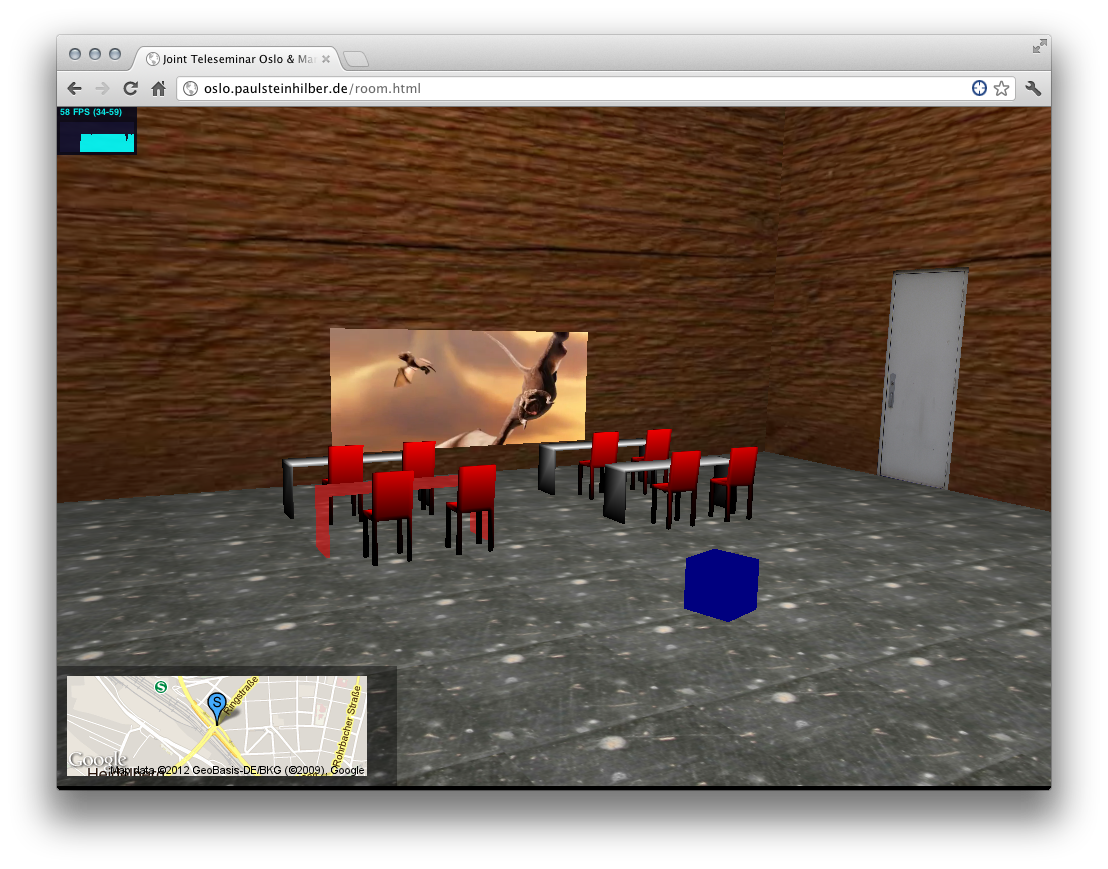
\includegraphics[width=\columnwidth]{grafiken/roomVideo}
	\caption{Room.html with playing video in Chrome on a desktop computer}
	\label{fig:roomVideo}
\end{figure}

\begin{figure}[htb]
	\centerline{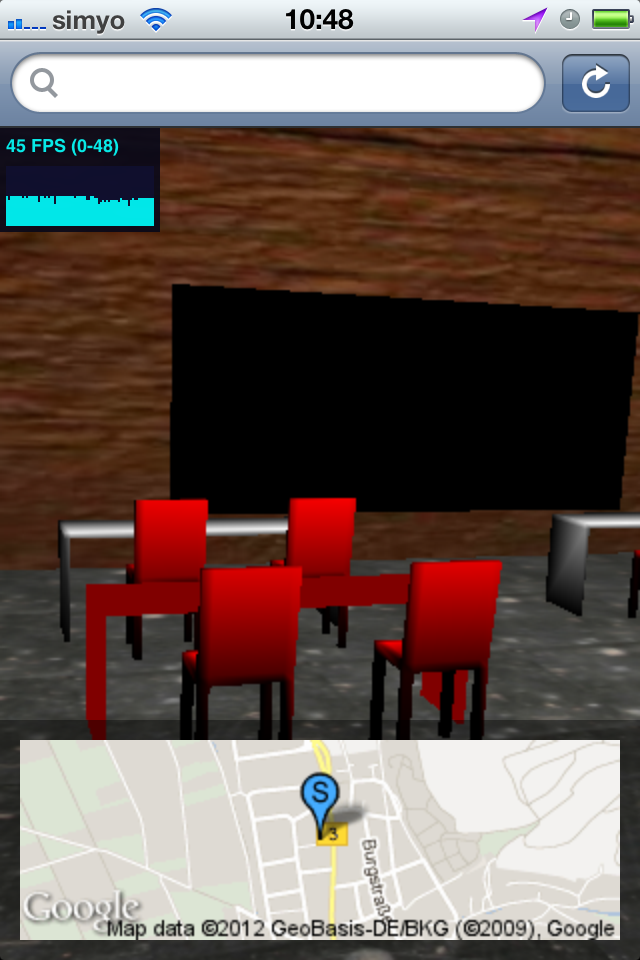
\includegraphics[width=0.6\columnwidth]{grafiken/room_Mobile}}
	\caption{Room.html shown in the WebGLViewer on an iPhone}
	\label{fig:roomMobile}
\end{figure}

The environment consists of a room with windows and a door (made of planes with textures) as well as several static and dynamic objects, i.e., chairs, tables, a blackboard, and a cube. Interaction is possible with some of them and they perform certain actions when clicked on or touched, i.e., the cube begins to rotate, the blackboard plays a video and a table displays further information.

The room is built using 6 planes put together to simulate a cube. Each plane has 4 vertices creating a single polygon. The blackboard is also of the simple sort. It is just a single plane and a single polygon. To make the windows and the door we added three additional planes with a texture, thus making the total number of polygons 9.

\subsubsection{Objects}
Objects in WebGL can both be build from scratch using basic shapes or can be imported from 3D modeling software. For our room we decided to use the tools provided by Three.js, a JavaScript 3D-library \cite{ThreeJS}, to create the "primitives" (basic geometric shapes such as a plane or a cube) and use Blender \cite{Blender3d}, an open source 3D application, for objects of greater complexity (such as the chairs and tables).

The blackboard is a simple plane consisting of 4 vertices which together create a polygon. As a texture for the blackboard we added a video element. The user can touch to interact with the blackboard which plays or pauses the video.

A single table contains 24 vertices which creates 22 polygons. Considering that our scene contains 4 tables, this means that the desks are responsible for 88 polygons. They all have a grey lambert material assigned with the exception of one table, which has a red basic material. This is to clearly show that it differs from the others and is interactive. When this table is touched a box appears explaining where such a table could be purchased.

A single chair consists of 56 vertices which results to 57 polygons. We have 8 chairs so this amounts to 456 polygons. All chairs have a red lambert material assigned, as no chair is interactive.

The cube is natively created in Three.js and consists of 8 vertices which amounts to 6 polygons. A basic red shader has been assigned similar to the other interactive objects. When the cube is touched it starts rotating and changes its color. Another touch stops the rotation and changes color one more time.

This gives us a grand total of 560 polygons in our application. 


\subsubsection{Interaction with Objects}
With the \textit{Ray} method/class the \textit{Three.js} library provides a simple method for interacting with 3D objects \cite{ThreeJSRay}. By specifying a starting point and the direction of the \textit{Ray}, any objects caught in the path of the ray will be added to an array. To identify these objects we have created an additional array holding all our "assigned" interactable objects. The starting point will always be the camera position and the direction is related to the mouse click or touch.
	We are only interested in the first interacted object (or else, in a larger project, we might be clicking on something in a separate room) and so it is the only object we bother comparing with our assigned interactable objects. When we have identified the object we perform the corresponding function.

\subsubsection{Textures}
Textures in the implementation were imported using \textit{THREE.ImageUtils.loadTexture()}, which creates a material based on the texture and combines it with the object. Although compressed textures are technically possible and are important for large applications, this technique was not used in this tech demo.

\subsubsection{Accessing Geolocation}
To demonstrate that it is possible to access the physical position of a mobile device with JavaScript we show a map of the device’s location at the bottom of the screen. 

To get the device’s location, the W3C Geolocation API \cite{locationAPI} was used. This API is independent from the underlying method to get the location. The location can be obtained from, for example GPS, or can be "inferred from network signals such as IP address, RFID, WiFi and Bluetooth MAC addresses, and GSM/CDMA cell IDs" \cite{locationAPI}. 

\subsubsection{Moving and Looking around in the Room}
Although data from a gyroscope is accessible with JavaScript and could be therefore used in a WebGL application, we have only used data provided by a device’s accelerometer, since not all of our test devices had a gyroscope included. The JavaScript \textit{onDeviceMotion}-event is used to get the accelerometer data. On iOS, "the accelerometer measures the sum of two acceleration vectors: gravity and user acceleration" \cite{CMDeviceMotion}. Using this data we were able to implement the feature to look up and down by moving the device. It is implemented in a way, that if the device is laying flat on a surface it shows the floor of the room. When holding the device vertically in your hand, you are looking at the blackboard.

The room application is reacting to touch events. You can swipe left or right to look to the left or the right, respectively.

If the application is run from a browser on a stationary machine or a laptop, it is possible to  move and look around in the room with the keyboard (W A S D and arrow keys). Alternatively, by pressing the left mouse button and while holding it pressed, moving the mouse, you can look around the room. Implementation of keyboard movements was done via one of \textit{Three.js} native movement classes since our endeavors to do so directly were rendered impossible by the lack of both documentation and complete implementation of the library \url{http://mrdoob.github.com/three.js/docs/48/#FlyControls}.

\section{Evaluation}
For the purpose of presenting the findings in our work in a structured and readily manner, we are going to devise a test matrix for our results. Since the WebGL technology is still relatively young and the support for it varies from browser to browser and from device to device, it would be very hard to devise common criteria for all the devices. Therefore,  we are approaching the problem by presenting the results separately for each device in the form Device - OS - Browser. In that way we can outline our observations in a much structured way and get to stress the peculiarities of WebGL support on different devices.

Since our goal is to investigate WebGL on mobile devices, we choose one desktop computer as a reference. Which OS (Mac OS, Windows or Linux) and particular machine (Mac or PC, laptop or a stationary) is used is not that important, since all the modern computers should be powerful enough to render WebGL graphics. The important thing is to choose a browser that fully supports WebGL. We find that Google Chrome is a good choice for that. All the measurements and observations will be taken running the \textit{Room.html}, as described in section \ref{roomhtml}, developed for the purpose of this paper.

Parameters we are observing are, for the most part, technical in nature. As the part of our application we are measuring Frames Per Second (FPS), parameter that gives us the number of times browser refreshes the screen per one second. In addition to the FPS we are also taking into consideration parameters like CPU usage and battery consumption, but as noted before the different parameters will be mentioned there it is applicable. 

Furthermore, in a similar approach to Golubovic \textit{et al.} \cite{Golubovic2011}, common functionality of WebGL is tested by executing the lessons of the WebGL tutorial from \url{learningWebGL.com} \cite{learningwebgl}. These lessons are based on a popular OpenGL tutorial (\textit{NeHe}, \url{nehe.gamedev.net/}) and cover most of the common functions, and should be enough to put our target devices to the test. The results of these tests are presented in table \ref{lessonsTable}.
 
In addition to technical parameters another interesting area of evaluation of WebGL is user experience. But since the most valid and exhaustive results in that field come from a large user surveys  \cite{Olsson2011b}, we are not going to do any work in that area.



\subsection{Energy Consumption}

\begin{table*}[tb]
	\begin{centering}
	\begin{tabular}{r|c|c|c|c|c|c}
		\multirow{2}{*}{\textbf{Test Case}} & \multicolumn{3}{c|}{\textbf{Battery and Energy Consumption}}						 & \multicolumn{3}{c}{\textbf{CPU Activity}}					\\
 							&\textbf{Time till 90\,\%} & \textbf{Battery Usage}	& \textbf{Relative Energy Usage} & \textbf{Total} 	& \textbf{Foreground App} 		& \textbf{Graphics}	\\
		\hline
		room.html		   &	36.03 min				& 0.278 $\frac{\%}{min}$	&	17							& 100\,\%			& 64\,\%						& 20\,\%			\\
		Quake 3			   &	34.67 min				& 0.289 $\frac{\%}{min}$	&	16							& 70\,\%			& 60\,\%						& 8\,\%			\\
		google.com		   &	78.93 min				& 0.127	$\frac{\%}{min}$	&	11							& 6\,\%				& 0.2\,\%						& 0.5\,\%		\\
	\end{tabular}
	\caption{Battery consumption and CPU activity of different WebGL applications\label{batteryTable}}
	\end{centering}
\end{table*}

\begin{figure}[htb]
	\centerline{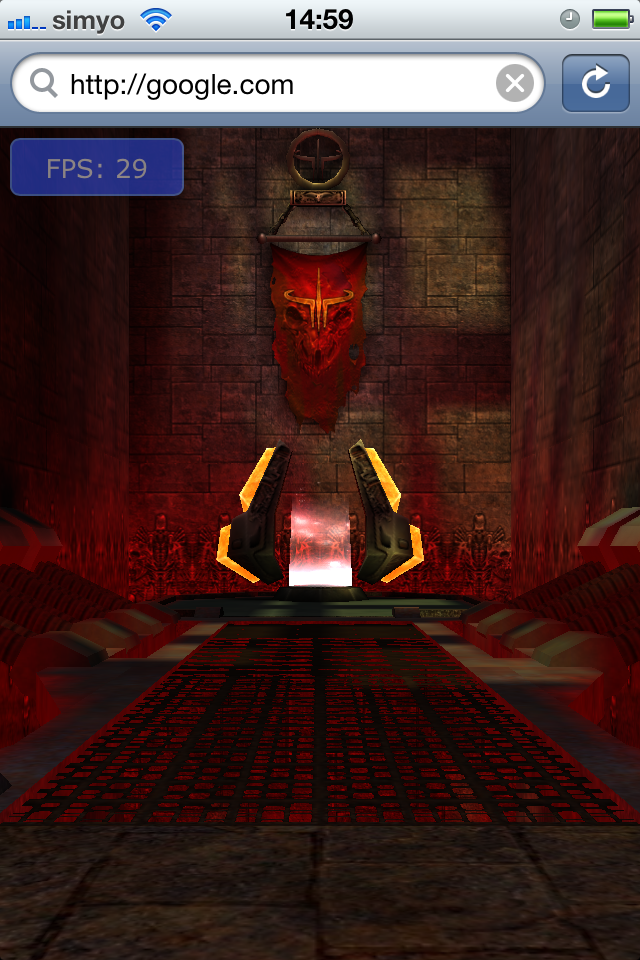
\includegraphics[width=0.6\columnwidth]{grafiken/quake3}}
	\caption{Quake 3 WebGL Demo \cite{quakewebgl} shown in the WebGLViewer on an iPhone}
	\label{fig:quake3}
\end{figure}

To measure the battery usage, the WebGLViewer application for iOS, as described in section \ref{WebGLViewer}, was used. The device was fully charged. The accordant content was opened in the WebGLViewer application. The device was then unplugged and the content reloaded. The time until the battery level decreased to 90\,\% as well as the battery consumption per minute was measured and calculated by the WebGLViewer. Using Apple Instruments, a part of Apple’s Developer Tools \cite{AppleDevTools}, we measured the \textit{CPU Activity} (\textit{Total Activity}, \textit{Foreground App Activity} and \textit{Graphics}) as well as the relative \textit{Energy Usage} on a scale from 0 to 20. All tests have been performed on an Apple iPhone 4 with iOS 5.1 installed using the WebGLViewer. We have compared the battery usage and CPU activity of the implemented \textit{Room.html}, the \textit{Quake 3 WebGL Demo} by Brandon Jones \cite{quakewebgl} (as shown in figure \ref{fig:quake3}) and \url{google.com} as reference. The results are shown in table \ref{batteryTable}.

Comparing the two WebGL applications to a normal website like \url{google.com} shows a huge difference in CPU activity. The overall CPU activity is below 10\,\%, with a value below 1\,\% for Foreground App Activity as well as \textit{Graphics Activity}, while using \url{google.com}, whereas the overall CPU activity is over 70\,\%, with about 60\,\% for \textit{Foreground App Activity} and up to 25\,\% for \textit{Graphics Activity}, while using a WebGL application. 

If we look at the battery consumption there is also a significant difference visible. The battery drains twice as fast while using a WebGL enabled website compared to \url{google.com}. The difference regarding the \textit{Relative Energy Usage} is not as big, however, we don't know how Apple calculates this value. \url{google.com} still needs less energy compared to the WebGL applications. Also the room.html has a higher \textit{Relative Energy Usage} compared to the Quake 3 WebGL Demo, which is consistent with our measurement of the battery usage, as well as with the time until the battery level decreases to 90\,\%.


\subsection{Frames per second}

\begin{figure}[htb]
	\centerline{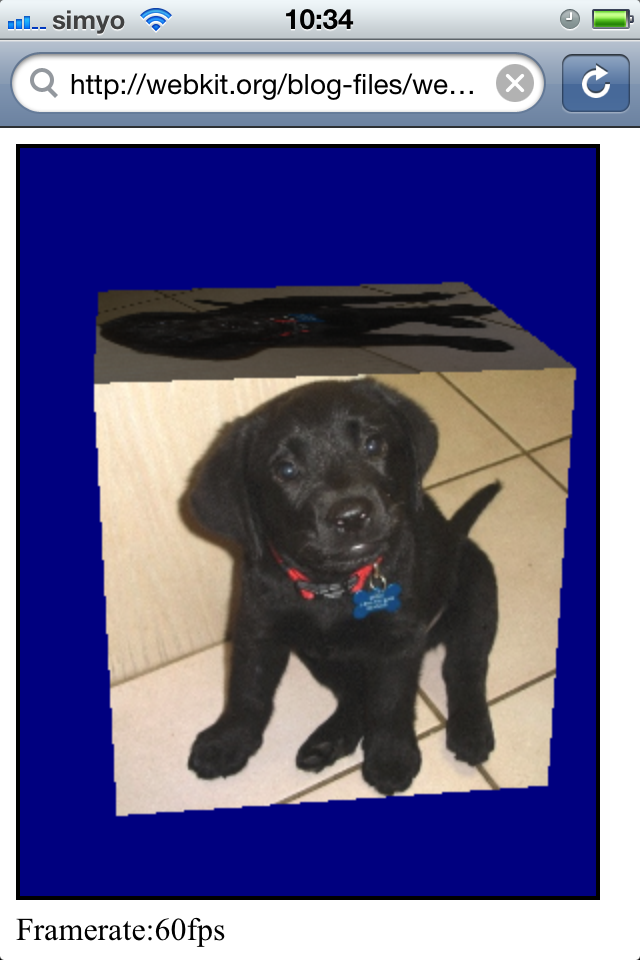
\includegraphics[width=0.6\columnwidth]{grafiken/SpiritBox}}
	\caption{WebGL demo SpiritBox by \cite{SpiritBox}}
	\label{fig:spiritbox}
\end{figure}

\begin{table*}[tb]
	\begin{centering}
	\begin{tabular}{l|l|l|l|l|l|l}
		\textbf{Device}	& \textbf{Operating System}	& \textbf{Browser}	& \textbf{Launched}	& \textbf{room.html}	& \textbf{Quake 3}	&	\textbf{SpiritBox}	\\
		\hline
		Apple iPad 2				& iOS 5.1			& WebGLViewer	& 2011		& 61 FPS	& 61 FPS	& 60 FPS		\\ 
		HTC EVO 3D					& Android 2.3.4		& Firefox		& 2011		& 8 FPS		& 12 FPS	& N/A $^{1}$	\\ 
		Apple iPhone 4				& iOS 5.1			& WebGLViewer	& 2010		& 40 FPS	& 29 FPS	& 43 FPS		\\
		Apple iPod Touch (4th Gen.)	& iOS 5.1			& WebGLViewer	& 2010		& 21 FPS	& 25 FPS	& 43 FPS		\\ 
%		HTC Desire					& Android 2.2.2		& Opera v12		& 2010		& 6 FPS 	&			&				\\ % room black == not working ???
		HTC Desire					& Android 2.2.2		& Firefox		& 2010		& 2 FPS 	& N/A		& 8 FPS			\\ % Mozilla == Firefox ??
		Apple iPhone 3GS			& iOS 5.1			& WebGLViewer	& 2009		&	36 FPS		&	27 FPS	&	60 FPS			\\
		\hline
		Reference Laptop $^{2}$			& 	Mac OS X 10.7.3			& 	Google Chrome	&	2010	&	34 FPS	&	36 FPS	&		50 FPS	\\
		Reference Computer $^{3}$		& 	Mac OS X 10.7.3			& 	Google Chrome	&	2006	&	58 FPS	&	59 FPS	&		85 FPS	\\
	\end{tabular}
	\caption{Frames per Second (FPS) of different WebGL applications on different devices\label{fpsTable}
	\\$^{1}$ \textit{The FPS value is constantly alternating between values in the range from 10 FPS up to over 200 FPS, making it impossible to determine a realistic value.}
	\\$^{2}$ \textit{Reference Laptop: MacBook 2010, Mac OS X 10.7.3, 2.26 GHz Intel Core 2 Duo, 4 GB DDR3 RAM}
	\\$^{3}$ \textit{Reference Computer: MacPro 2006, Mac OS X 10.7.3, 2x 2.0 GHz Dual-Core Intel Xeon, 6 GB DDR2 RAM}}
	\end{centering}
\end{table*}

To test the performance of WebGL on different platforms we have measured and compared frames per second (FPS) for different applications. FPS describes the frequency at which images are generated. The values below 10-12 FPS, are recognizable by the human eye as the separate images; for higher FPS, single images cannot be recognized and they blend together creating motion \cite{12FPS}. So a higher number of FPS creates a more fluid animation and is therefore considered better. Since the refresh rate of modern flat screens is 60 FPS there is usually no need to render with more than 60 FPS \cite{60fps}.

In table \ref{fpsTable} we compared the FPS of the implemented \textit{Room.html}, the \textit{Quake 3 WebGL Demo} \cite{quakewebgl} (as shown in figure \ref{fig:quake3}), and an example of a spinning cube, the \textit{SpiritBox} from \url {webkit.org} \cite{SpiritBox} (as shown in figure \ref{fig:spiritbox}), on different mobile devices as well as on one laptop computer (2010 MacBook) and stationary computer (2006 MacPro) as reference. 

\begin{table*}[tb]
	\begin{centering}
	\begin{tabular}{l|l|l|l|l|l|l|l}
		\textbf{Lesson}								& \textbf{Reference$^{1}$}& \textbf{Desire}		& \textbf{EVO 3D}		& \textbf{iPhone 4}		& \textbf{iPhone 3GS}	& \textbf{iPad 2}	& \textbf{iPod Touch}\\
		\hline
		3 - Simple animations						& 59 FPS		& 13 FPS		& 16 FPS		& 57 FPS		& 57 FPS		& 58 FPS	& 40 FPS				\\
		4 - 3D animations							& 58 FPS		& 12 FPS		& 19 FPS		& 57 FPS		& 57 FPS		& 58 FPS	& 57 FPS				\\
		5 - Textures								& 59 FPS		& 13 FPS		& 16 FPS		& 40 FPS		& 57 FPS		& 58 FPS	& 40 FPS				\\
		6 - Texture filters and keyboard			& 59 FPS		& 12 FPS		& 18 FPS		& 40 FPS		& 57 FPS		& 58 FPS	& 40 FPS				\\
		7 - Basic Lighting							& 59 FPS		& 12 FPS		& 17 FPS		& 57 FPS		& 57 FPS		& 58 FPS	& 57 FPS				\\
		8 - Transparency and blending				& 59 FPS		& 11 FPS		& 16 FPS		& 58 FPS		& 57 FPS		& 58 FPS	& 58 FPS				\\
		9 - Particles								& 59 FPS		&  8 FPS		& 17 FPS		& 39 FPS		& 31 FPS		& 60 FPS	& 40 FPS				\\
		10 - Loading a map							& 58 FPS		& 11 FPS		& 15 FPS		& 57 FPS		& 57 FPS		& 58 FPS	& 40 FPS				\\
		11 - Sphere and rotation					& 59 FPS		& 12 FPS		& 15 FPS		& 40 FPS		& 57 FPS		& 58 FPS	& 57 FPS				\\
		12 - Point lighting							& 58 FPS		& 11 FPS		& 15 FPS		& 40 FPS		& 57 FPS		& 58 FPS	& 40 FPS				\\
		13 - Per-fragment lighting					& 59 FPS		& 10 FPS		& 17 FPS		& 36 FPS		& 40 FPS		& 58 FPS	& 39 FPS				\\
		14 - Specular highlights and JSON model		& 58 FPS		&  9 FPS		& 15 FPS		& 35 FPS		& 39 FPS		& 58 FPS	& 36 FPS				\\
		15 - Specular maps							& 58 FPS		&  8 FPS		& 16 FPS		& 22 FPS $^{2}$	& 24 FPS $^{2}$	& 58 FPS $^{2}$	& 22 FPS $^{2}$ 		\\
		16 - Render to texture						& 58 FPS		&  6 FPS		& 16 FPS		& 22 FPS		& 22 FPS		& 58 FPS	& 22 FPS				\\
	\end{tabular}
	\caption{Frames per Second (FPS) using the lessons from the learning WebGL tutorial on different devices\label{lessonsTable}
	\\\textit{$^{1}$ Reference Computer: MacBook 2010, Mac OS X 10.7.3, 2.26 GHz Intel Core 2 Duo, 4 GB DDR3 RAM}
	\\\textit{$^{2}$ Rendering results aren't looking as expected}
	}
	\end{centering}
\end{table*}

\begin{figure}
	\centerline{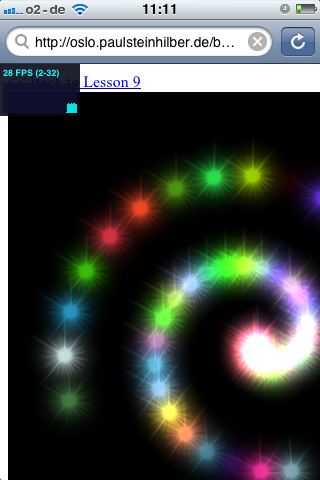
\includegraphics[width=0.6\columnwidth]{grafiken/lesson9}}
	\caption{"Lesson 9" WebGL demo (adapted from \cite{lesson9})}
	\label{fig:lesson9}
\end{figure}

The lessons from \url{learningWebGL.com} \cite{learningwebgl} have been used as a benchmark to test the performance on different mobile device. As example figure \ref{fig:lesson9} shows a screenshot of lesson 9. The results are shown in table \ref{lessonsTable}.

Opera has advertised the WebGL capabilities beginning with Opera Mobile 12 \cite{opera12}, but the performance of WebGL content on this browser is much worse than in Firefox. Although all lessons from table \ref{lessonsTable} are rendered correctly, the frame rate was always below 10 FPS, compared with 16 FPS in average in Firefox on the HTC EVO 3D. The \textit{SpiritBox} on the other hand is not rendered correctly (only a blue square is visible) and the room.html doesn’t load at all.

The most obvious result is the big performance difference between the iOS and Android devices. Even the HTC EVO 3D, which was launched in 2011, was not able to deliver results comparable to the iPhone 3GS launched in 2009. On the Android devices the \textit{Room.html} was unusable to interact with fluidly, whereas it was rendered smoothly on all iOS devices. 

While the Android devices have always had lower frame rates compared to the iOS devices, they were able to render all lessons from table \ref{lessonsTable} correctly. iOS based  devices, on the other hand, were not able to render lesson 15 correctly. Screenshots to compare the rendering of lesson 15 on Android and iOS are shown in figure \ref{fig:lesson15_Android} and figure \ref{fig:lesson15_iOS}, respectively. 

\begin{figure}[htb]
	\begin{center}
	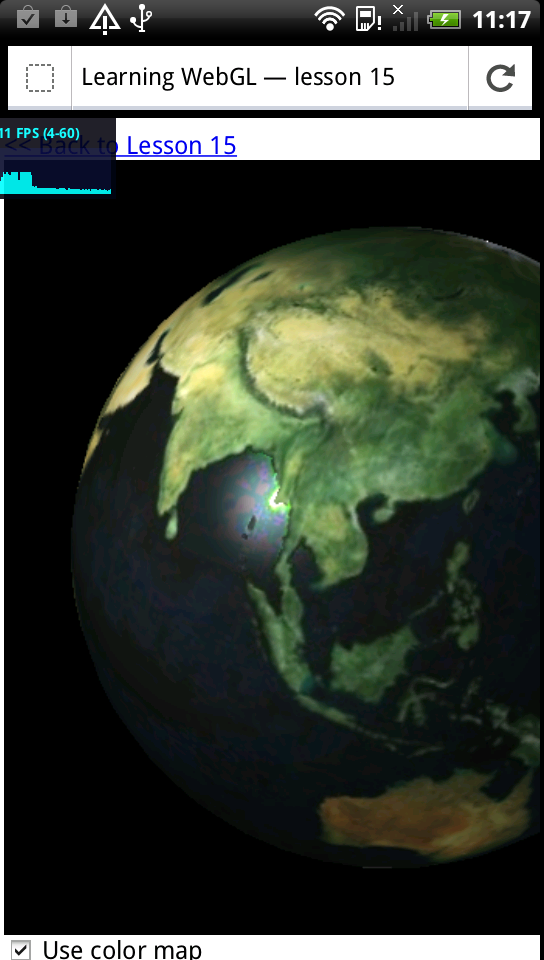
\includegraphics[width=0.65\columnwidth]{grafiken/lesson15_Android}
      \caption{"Lesson 15" WebGL demo on Android (adapted from \cite{lesson15})}
      \label{fig:lesson15_Android}
    \end{center}
\end{figure}

\begin{figure}[htb]
	\begin{center}  
    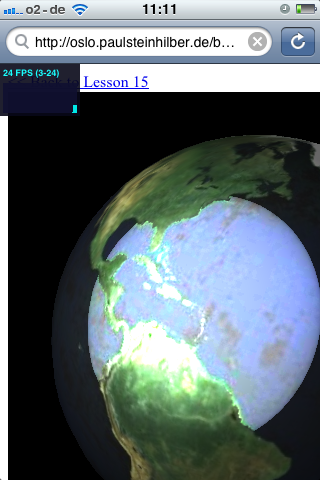
\includegraphics[width=0.6\columnwidth]{grafiken/lesson15_iOS}
      \caption{"Lesson 15" WebGL demo on iOS (adapted from \cite{lesson15})}
      \label{fig:lesson15_iOS}
    \end{center}
\end{figure}

Another interesting result is, that the iPhone 3GS delivers significantly higher frame rates in some tests compared to the iPhone 4. An possible explanation could be, that the iPhone 4’s display resolution is significantly higher, thus requiring the calculation of four times more pixels. 

%explicit answer to both q1 and q2
Comparing the performance of our reference machine, the 2010 MacBook, with the iOS based mobile devices is an indicator that today's mobile devices are powerful enough to render 3D applications with an acceptable frame rate.

\subsection{Limitations}
Albeit most of the tests we have performed were successful, we have still encountered a few limitations during our test phase. We are listing them, further down the text.

\subsubsection{Device Sensors Access}\label{deviceSensors}
WebRTC, an upcoming standard for access to the device’s video camera and microphone, is currently only available on Opera Mobile 12, a browser currently not supported on iOS. With the Android devices lacking in performance, we were unable to implement a WebRTC application.

During our evaluation and testing on other devices, we realized that the accelerometer wasn’t working as intended on Android using a HTC EVO 3D running the \textit{Room.html} in Firefox. When the device is laying flat on a surface, the room’s floor is shown as expected. Holding it vertically in your hand, however, still shows the floor. The accelerometer is undoubtedly working, but it seems to be much less sensitive, than the one on iOS based devices. Therefore, the feature to look up and down with the accelerometer is deactivated, when non-iOS device is detected.

\subsubsection{Key and Mouse Events}
As expected, key and mouse events cannot be triggered in WebGL on mobile devices with touch screens, but replacing them with touch events is a working solution for this problem.

\subsubsection{Video texture}
Touching the blackboard should start playing a movie on it. It worked perfectly on desktop computers using Windows, Mac and Linux as operating systems and Chrome, Safari and Firefox as browsers. We were unable to get the video texture working correctly on the mobile devices, though.

Namely, neither audio nor video were reproduced on the mobile devices after touching the blackboard, with the exception of working audio on the iPad 2. Using an iPhone 4 a significant decrease of the frame rate could be observed after tapping the blackboard. The frame rate dropped from 47 FPS to just 20 FPS after touching the blackboard. While measuring the CPU activity, after tapping the blackboard, the \textit{Foreground App Activity} dropped from about 60\,\% to 30\,\% while the \textit{Audio Processing} increased from 0\,\% to about 10\,\%, with an overall CPU activity of 100\,\% on an iPhone 4.

The video played perfectly using just the HTML5 video tag on iOS using Safari or WebGLViewer, hence a wrong video encoding could be eliminated as source of the problem. Since the video texture works on all browsers and all desktop operating systems, and the video’s audio is even played on the iPad 2, we are assuming that our implementation is correct. 

Therefore we think, that video texture not working for us is actually a limitation of WebGL on mobile devices.


\section{Conclusion}
In this paper we developed an application with the purpose of testing the feasibility of augmented reality (specifically 3D-augmentation) on mobile devices using only a web browser. 

The technical possibilities for accessing the device’s sensors for interacting with the user’s context, crucial to develop AR applications, are now given, even though in an early phase. One of the most common properties associated with augmented reality is camera integration, and although it is technically possible to realize this using pre-alpha software, due to the limitations of the mobile devices we tested (as mentioned in section \ref{deviceSensors}), we were not able to test augmented reality in a browser using a camera. Other requirements for augmented reality applications on mobile devices were successfully shown.

As we can see from the results, there was a huge difference between iOS and Android with regards to performance, but both seemed to handle the task, though with certain limitations as discussed previously. The application renders on all our devices, and some basic user interaction is possible. Compared to a reference machine we saw that the rendering cycle expressed through the FPS is a bit lower on mobile devices, but still good (with exception of Apple’s iPad 2, whose frame rate is comparable to the one on our reference machine). Furthermore, we observed that battery consumption is relatively high while running WebGL applications compared to ordinary web-surfing. 

Our results, presented in this paper, indicate that WebGL at its current state can be used on mobile devices to augment 3D objects to a user’s view. The standards for AR applications in web browsers are not yet completed, and implementations are not stable yet,  which makes a widespread use nearly impossible at this moment. However, if Moore’s law \cite{Schaller1997} applies to the progression of mobile devices as well as web standards, and mobile software continue to follow its current pace, we can be sure that augmented applications in web browsers could be ubiquitous on mobile devices in the near future.





\appendices
\section*{Installing WebGLViewer}
To install the WebGLViewer using the provided source code on an iOS device a membership in Apple's iOS Developer Program is needed. However compiling and running the WebGLViewer in the iOS Simulator is possible using XCode. As alternative, a registered developer can provide you a binary, which is build for your specific device. We used \url{testflight.com} to distribute such binaries. To request a binary you need to create an account on \url{http://bit.ly/zWoZQJ} and register your device as soon as you are accepted.



\ifCLASSOPTIONcaptionsoff
  \newpage
\fi



\bibliographystyle{IEEEtran}
\bibliography{bib}

\end{document}


